\section{Filter}
\textbf{HAREC a.\ref{HAREC.a.3.2}\label{myHAREC.a.3.2}}
\index{filter}
\index{filter!frekvensfilter}

%% sid II3-7/138

Frekvensfilter, eller mer allmänt filter, används inom radiotekniken för många
olika ändamål, t.ex. för att
\begin{itemize}
\item eliminera störande signaler,
\item  öka avstämningsskärpan (selektiviteten) i mottagare och sändare,
\item framhäva eller dämpa ett sidband i en AM-signal m.m.
\end{itemize}

Beroende på den s.k. frekvensgången, så indelas filtren i flera ''familjer'',
varav de vanliga presenteras här.

Beroende på det tekniska utförandet finns dels s.k. passiva filter vilka
använder extern energi för sin funktion, och dels aktiva filter vilka i princip
är förstärkare som likaledes använder passiva kretsar. Här presenteras
för enkelhetens skull passiva filter.

Traditionella frekvensfilter är vad som kallas analoga. Men nu i dataåldern
börjar även digitala filter vinna intåg. Sådana är dock för komplicerade för
att behandlas här.

\subsection{Högpassfilter (HP)}
\textbf{HAREC a.\ref{HAREC.a.3.2.8b}\label{myHAREC.a.3.2.8b}}
\index{högpassfilter}
\index{filter!högpass (HP)}
\index{highpass filter}
\index{HP}

\begin{figure}
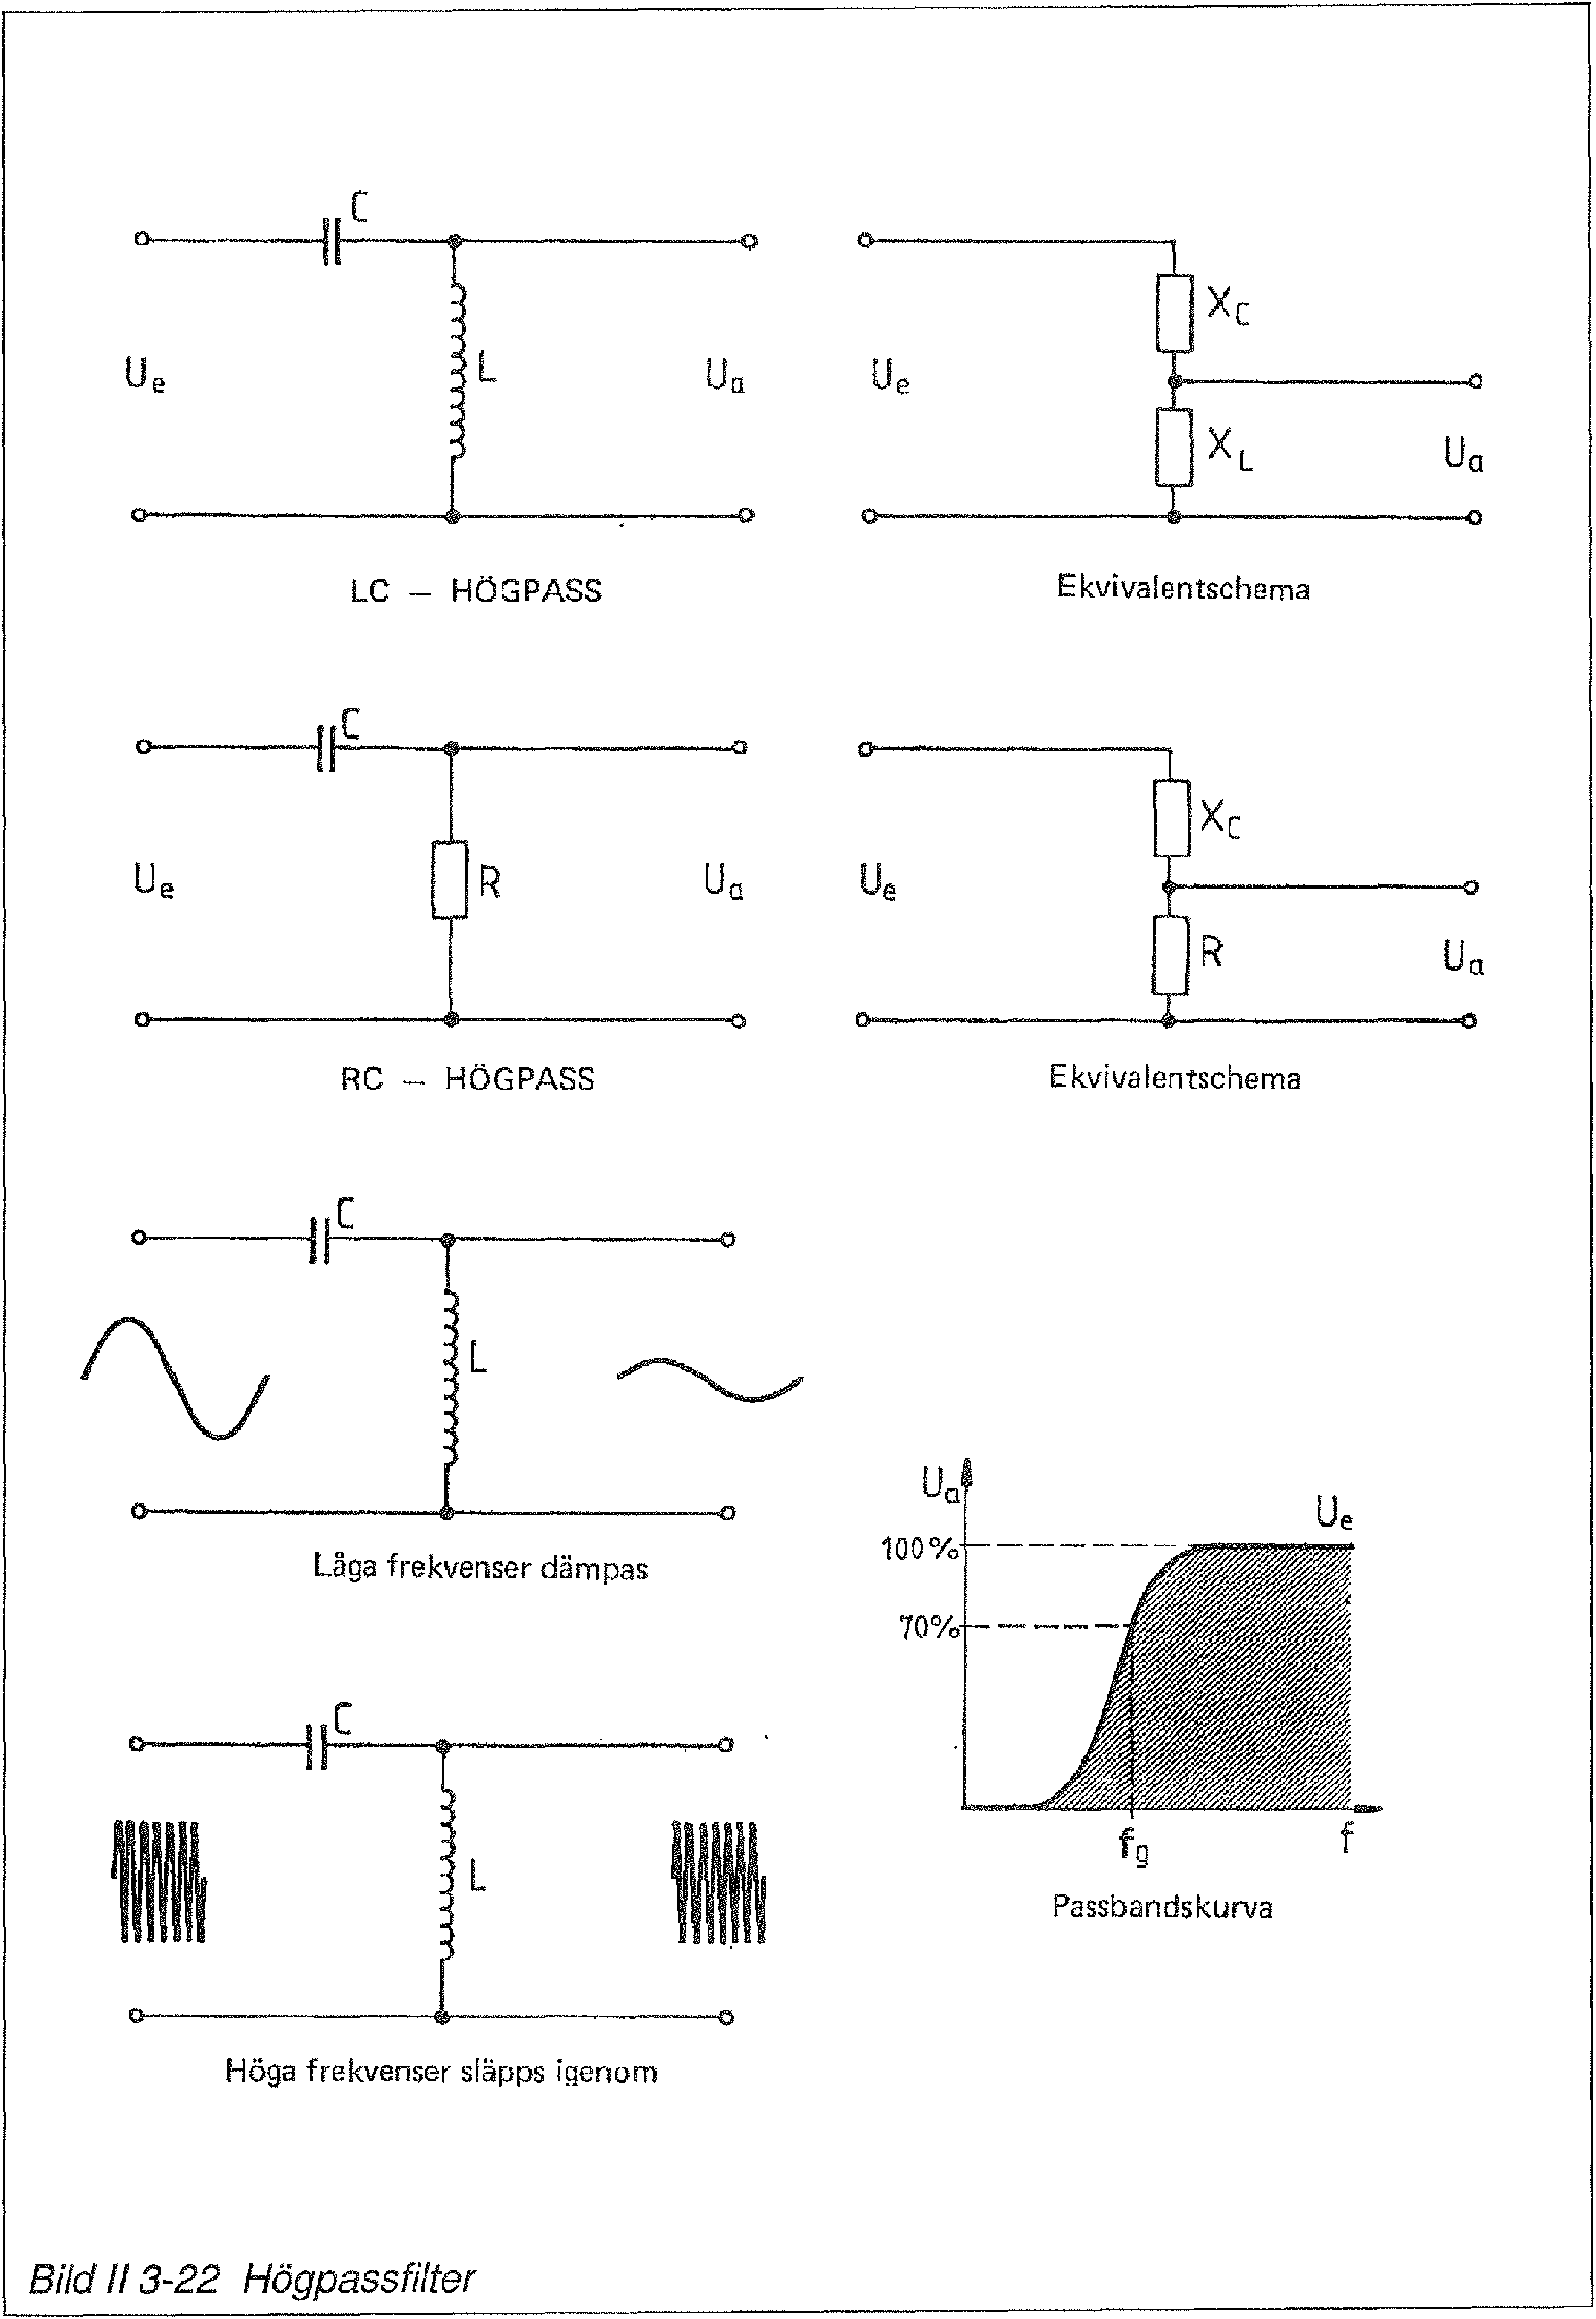
\includegraphics[width=\textwidth]{images/bild_2_3-22}
\caption{Högpassfilter}
\label{fig:BildII3-22}
\end{figure}

Bild \ref{fig:BildII3-22}

Ett \emph{högpassfilter} (eng \emph{highpass filter (HP)}) släpper igenom
signaler med höga frekvenser och dämpar dem med låga frekvenser.

Exempel: En frekvensberoende spänningsdelare som LC-högpassfilter.

Vid låga frekvenser är \(X_C\) stor och \(X_L\) liten. Över XL uppstår då ett
litet spänningsfall - en låg utgångsspänning \(U_a\). Resultatet blir att
låga frekvenser dämpas.

Vid höga frekvenser är \(X_C\) liten och \(X_L\) stor. Över \(X_L\) uppstår då
ett stort spänningsfall- en hög utgångsspänning \(U_a\). Resultatet blir att
höga frekvenser släpps igenom.

\(X_L\) kan bytas ut mot en resistor \(R\), men då blir passbandkurvan inte så
brant.

\emph{Gränsfrekvens}

Gränsfrekvensen \(f_g\) beror av kapacitansen \(C\), induktansen \(L\) samt
resistansen \(R\).

LC-högpass:
\begin{gather*}
  f_g = \frac{1}{2π\sqrt{LC}} \\
  f_g\ \text{[Hz]} \quad L\ \text{[H]} \quad C\ \text{[F]}
\end{gather*}

RC-Högpass:
\begin{gather*}
  f_g = \frac{1}{2πRC}
  f_g\ \text{[Hz]} \quad R\ \text{[Ω]} \quad C\ \text{[F]}
\end{gather*}

Räkneexempel:
\begin{enumerate}
\item \(L = 4\ \text{H} \quad C = 1\ \text{µF} \quad f_g =\ ?\)
  \[
  f_g = \frac{1}{2π\sqrt{4 \cdot 10^{-6}}} = \frac{500}{2π}
  = 79,6\ \text{Hz}
  \]
\item \(R = 1\ \text{kΩ} \quad C = 10\ \text{nF} \quad f_g =\ ?\)
  \[
    f_g = \frac{1}{2π \cdot 1 \cdot 10^3 \cdot 10 \cdot 10^{-9}}
    = \frac{10^5}{2π} = 15,9\ \text{kHz}
  \]
\end{enumerate}

\subsection{Lågpassfilter (LP)}
\textbf{HAREC a.\ref{HAREC.a.3.2.8a}\label{myHAREC.a.3.2.8a}}
\index{lågpassfilter}
\index{filter!lågpass (LP)}
\index{lowpass filter}
\index{LP}

\begin{figure}
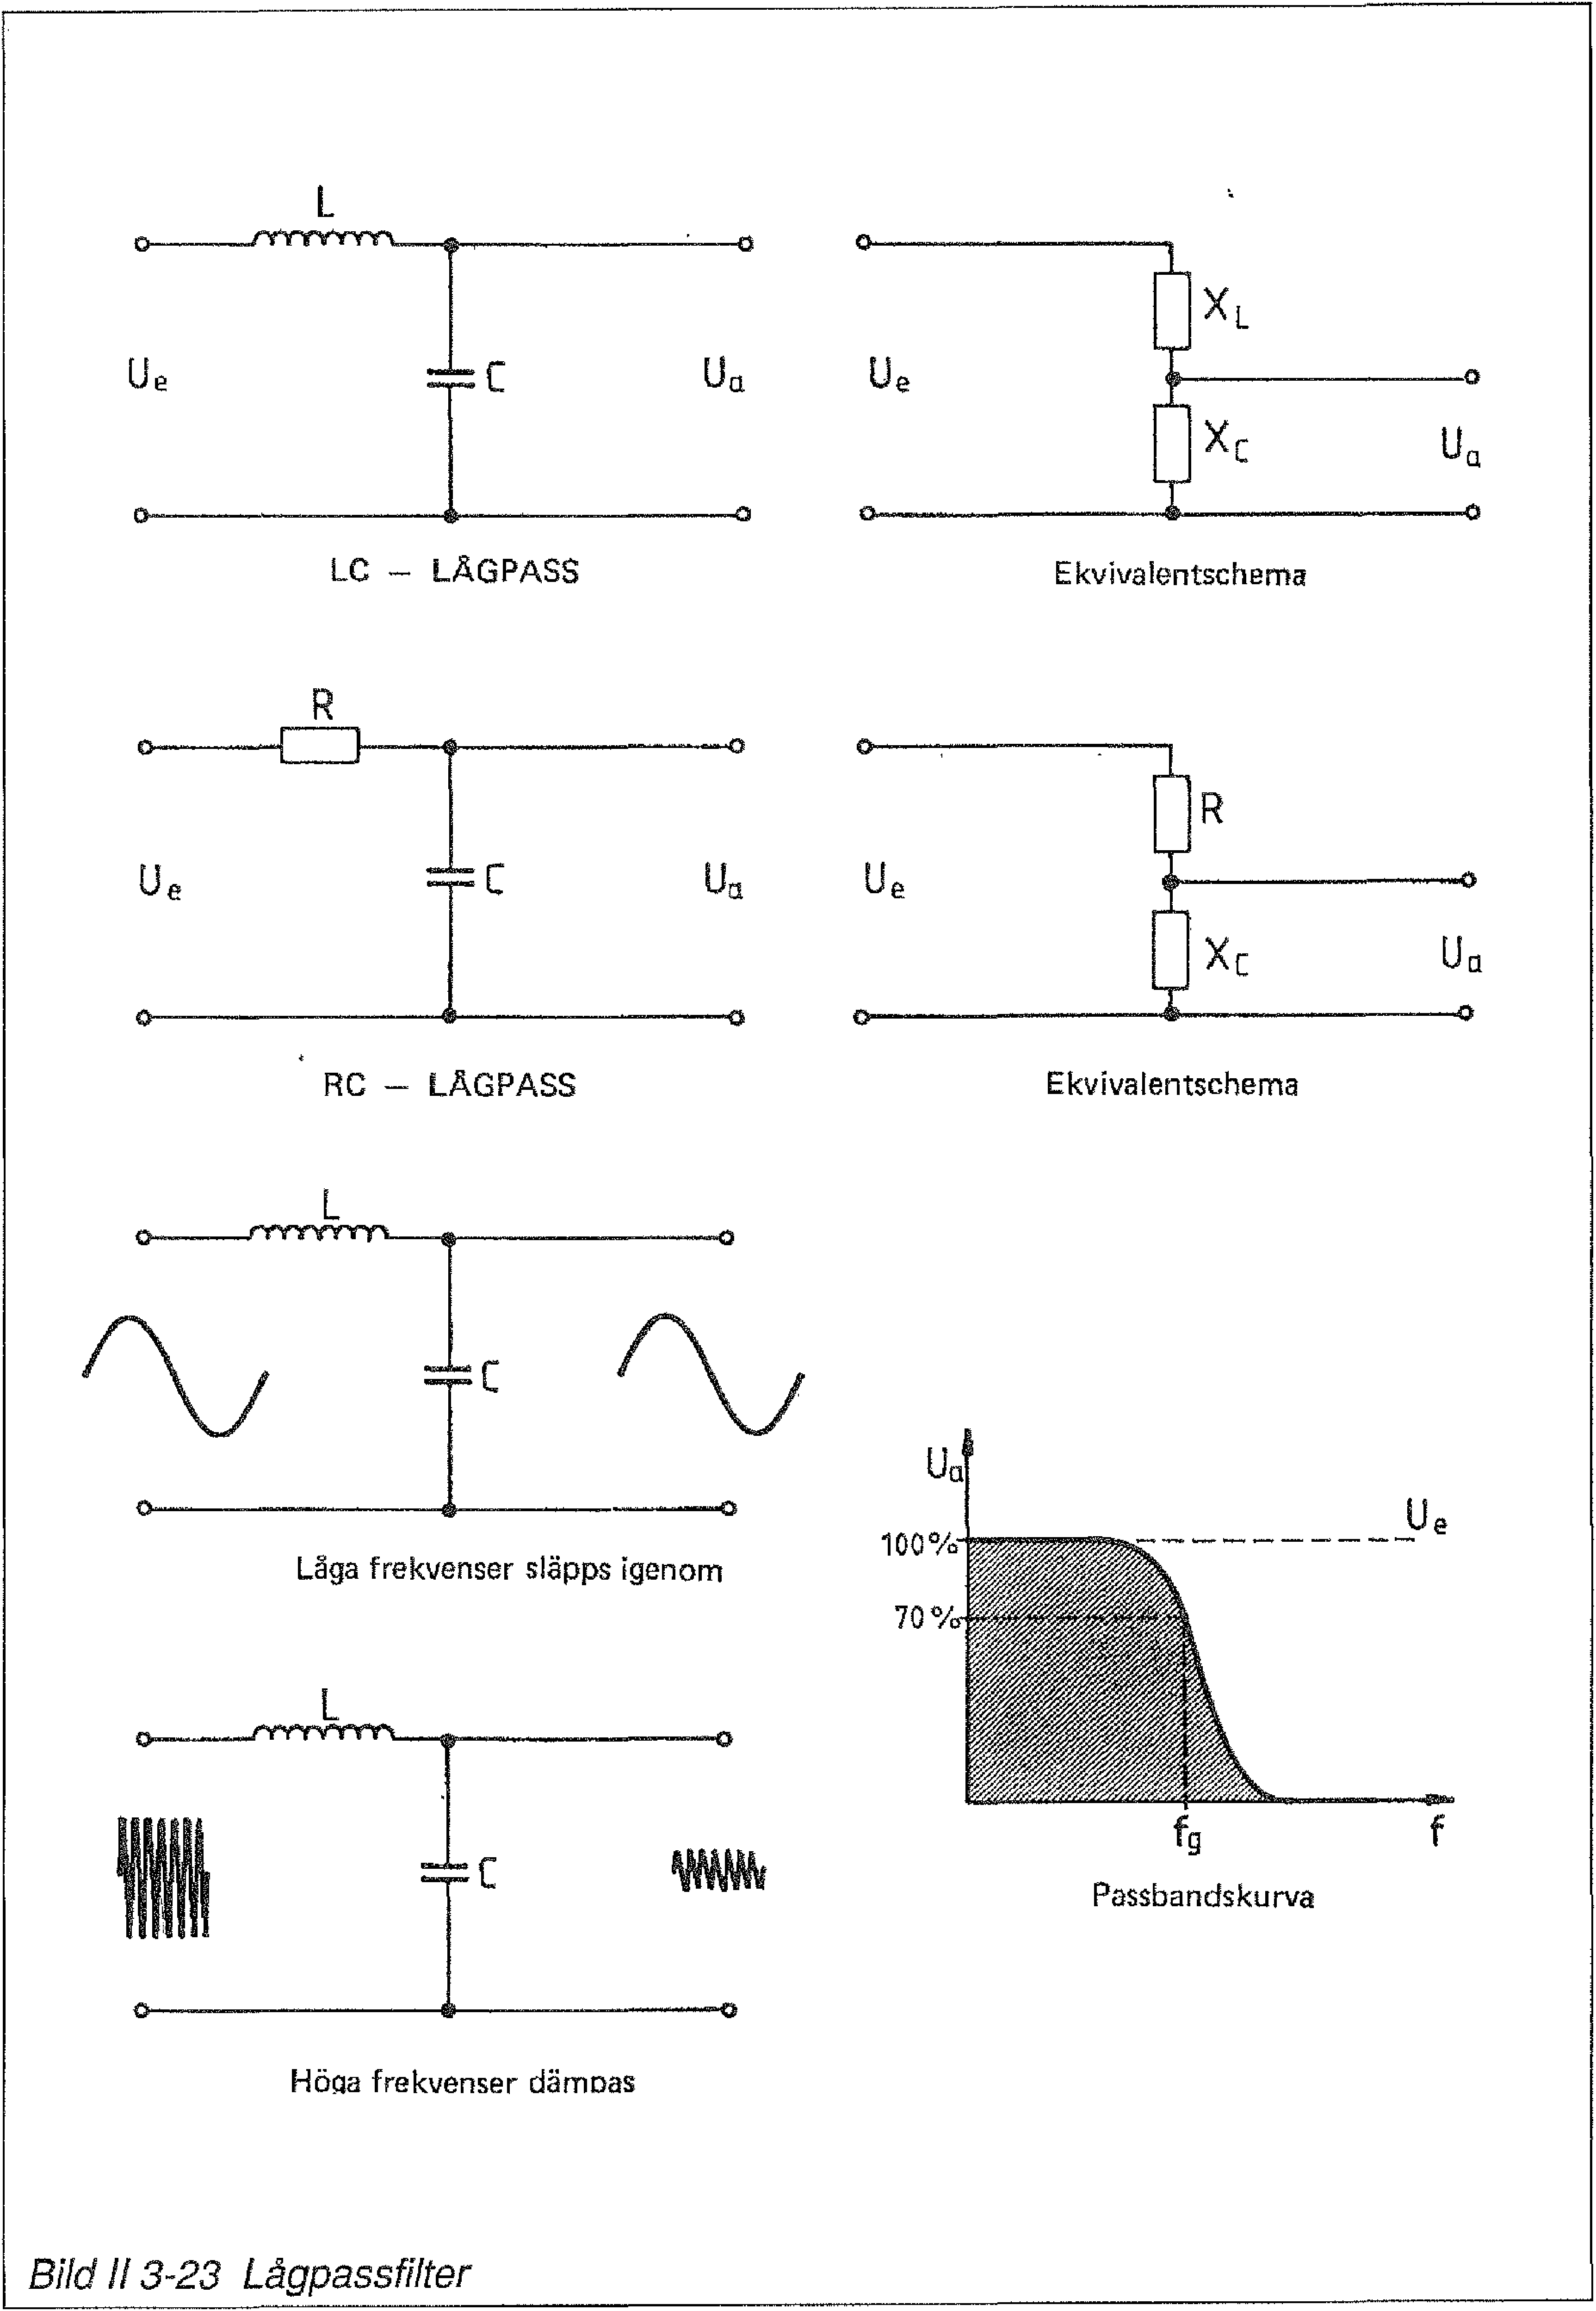
\includegraphics[width=\textwidth]{images/bild_2_3-23}
\caption{Lågpassfilter}
\label{fig:BildII3-23}
\end{figure}

Bild \ref{fig:BildII3-23}

Om induktor och kondensator respektive resistor och kondensator i ett
högpassfilter byter plats, så får man i stället ett LC-lågpassfilter respektive
ett RC-lågpassfilter.

Ett \emph{lågpassfilter} (eng \emph{lowpass filter (LP)}) släpper igenom
signaler med låga frekvenser och dämpar dem med höga frekvenser.

Exempel: En frekvensberoende spänningsdelare som LC-Lågpassfilter.

Vid låga frekvenser är \(X_C\) stor och \(X_L\) liten. Över \(X_L\) uppstår då
ett litet spänningsfall - en hög utgångsspänning \(U_a\). Resultatet blir att
låga frekvenser släpps igenom.

Vid höga frekvenser är \(X_C\) liten och \(X_L\) stor. Över \(X_L\) uppstår då
ett stort spänningsfall - en låg utgångsspänning \(U_a\). Resultatet blir att
höga frekvenser dämpas.

\emph{Gränsfrekvens}

Samma formler används vid beräkning av gränsfrekvensen både i lågpass- och
högpassfilter, således

LC-Lågpass:
\begin{gather*}
  f_g = \frac{1}{2π\sqrt{LC}} \\
  f_g\ \text{[Hz]} \quad L\ \text{[H]} \quad C\ \text{[F]}
\end{gather*}

RC-Lågpass:
\begin{gather*}
  f_g = \frac{1}{2π{RC}} \\
  f_g\ \text{[Hz]} \quad R\ \text{[Ω]} \quad C\ \text{[F]}
\end{gather*}

\subsection{Bandpassfilter (BP)}
\textbf{HAREC a.\ref{HAREC.a.3.2.8c}\label{myHAREC.a.3.2.8c}}
\index{bandpassfilter}
\index{filter!bandpass (BP)}
\index{bandpass filter}
\index{BP}

\begin{figure}
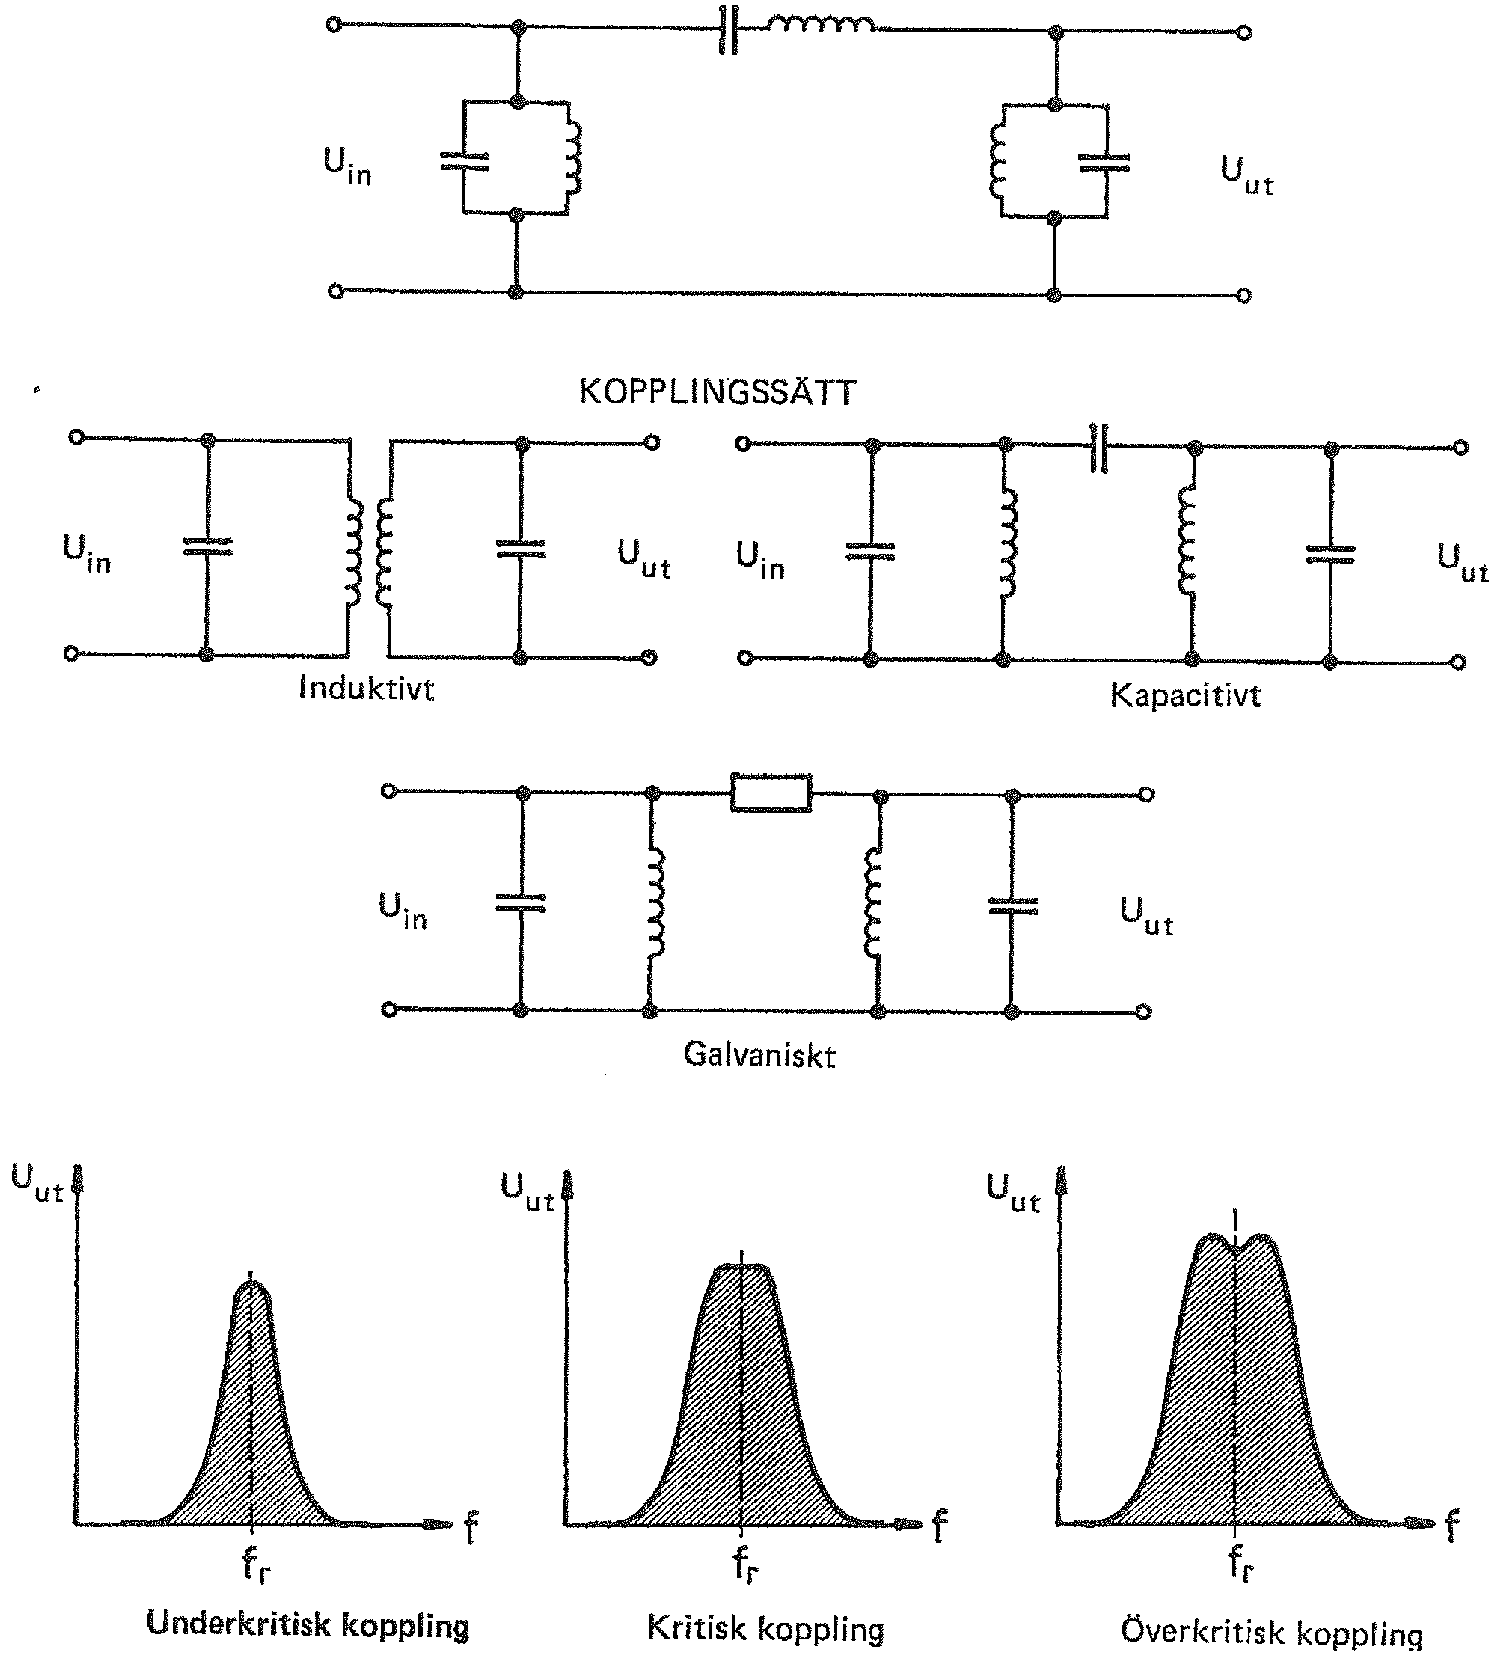
\includegraphics[width=\textwidth]{images/bild_2_3-24}
\caption{Bandpassfilter}
\label{fig:BildII3-24}
\end{figure}

Bild \ref{fig:BildII3-24}

Ett bandpassfilter släpper igenom signaler bara inom ett frekvensområde medan
signaler inom andra frekvensområden dämpas.

Bandpassfiltret består i enklaste fall av två svängningskretsar av LC-typ, vilka
är avstämda till angränsande frekvenser. Kretsarna är kopplade induktivt,
kapacitivt eller galvaniskt.

Beroende på kopplingsgrad skiljer man mellan underkritisk koppling (lös
koppling), kritisk koppling och överkritisk koppling (fast koppling).

På bilden visas hur passbandet påverkas bl.a. av kopplingsgraden. Lös koppling
liten bandbredd. Kritisk koppling - större bandbredd. Fast koppling - stor
bandbredd.

\subsection{Passfilter}
\index{passfilter}
\index{filter!bandpass (BP)}
\index{pass filter}
\index{BP}

\begin{figure}
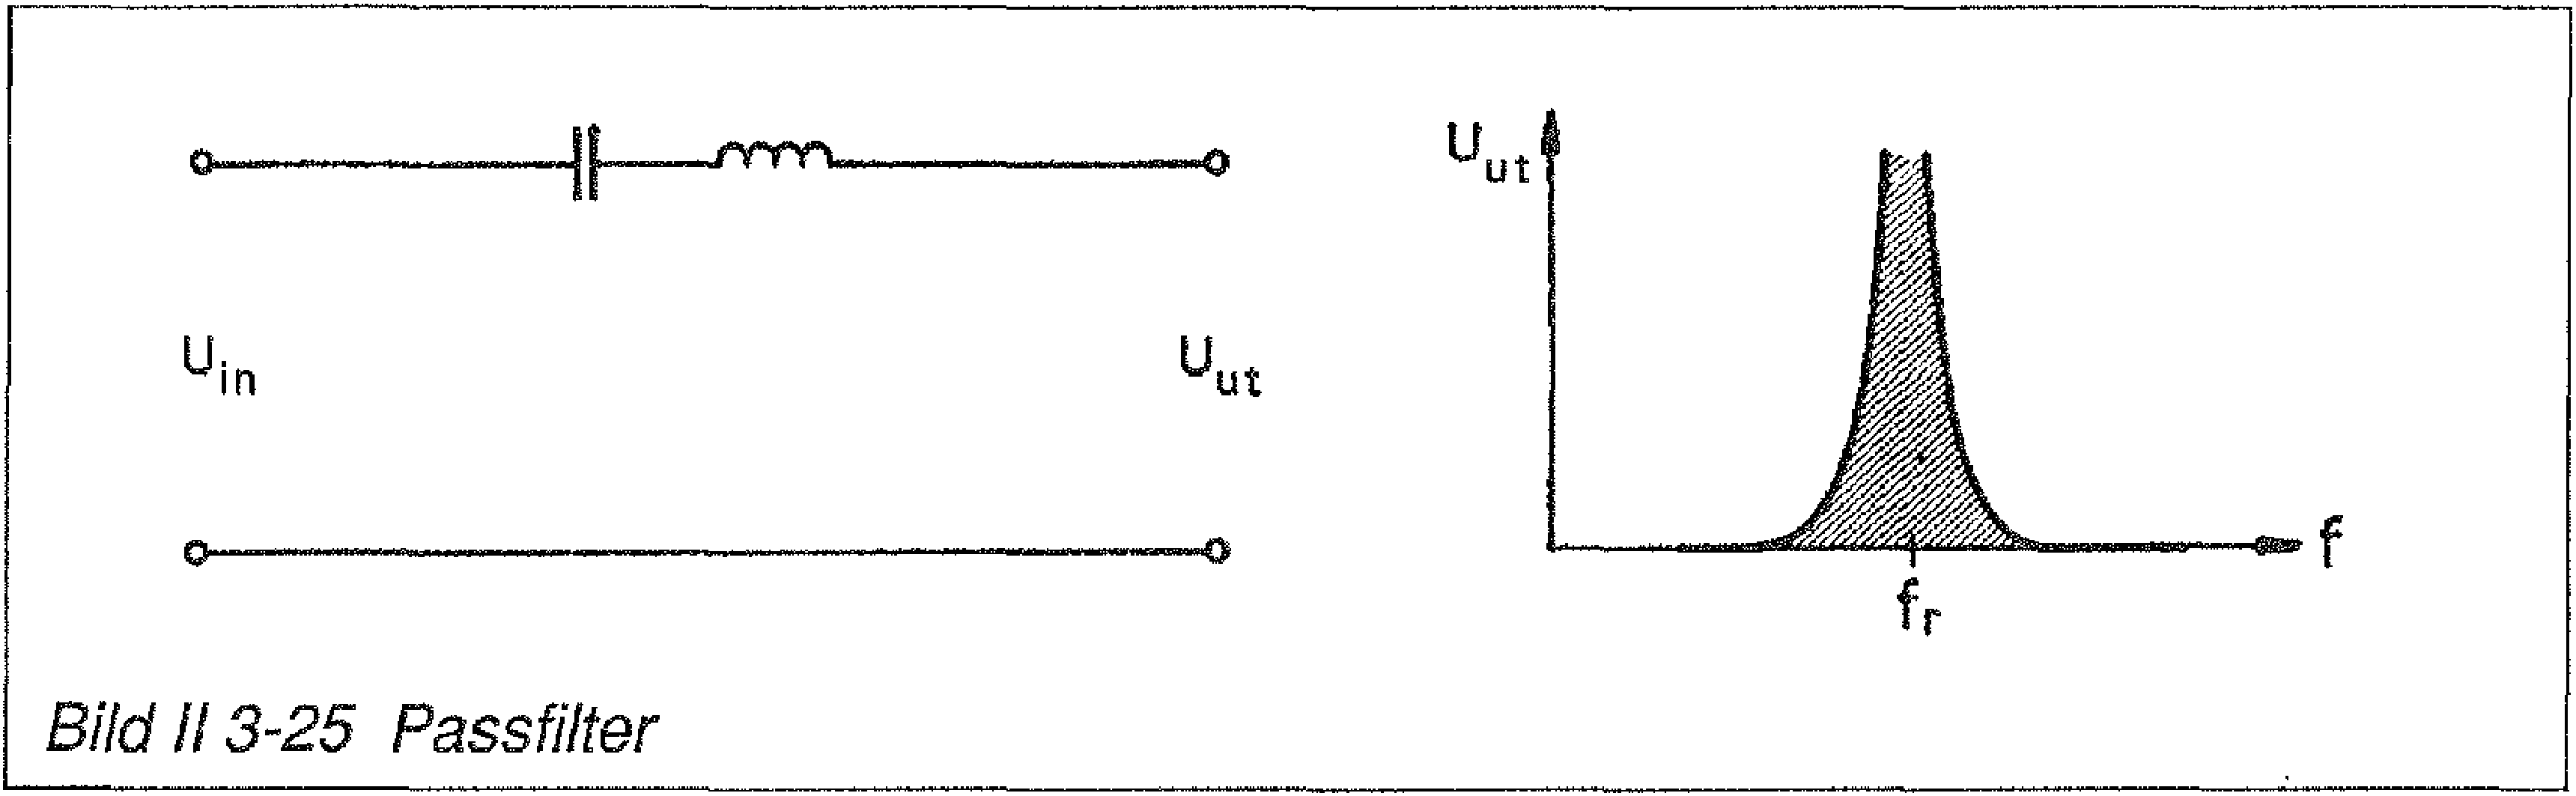
\includegraphics[width=\textwidth]{images/bild_2_3-25}
\caption{Passfilter}
\label{fig:BildII3-25}
\end{figure}

Bild \ref{fig:BildII3-25}

Passkretsen stäms av till en viss frekvens och erbjuder där en mycket låg
impedans. Passkretsen kopplas i serie med signalvägen och låter signaler med
frekvenser inom filtrets passband att passera.

\subsection{Bandspärrfilter}
\textbf{HAREC a.\ref{HAREC.a.3.2.8d}\label{myHAREC.a.3.2.8d}}
\index{bandspärrfilter}
\index{filter!bandspärr (BR)}
\index{band reject filter (BR)}
\index{BR}

\begin{figure}
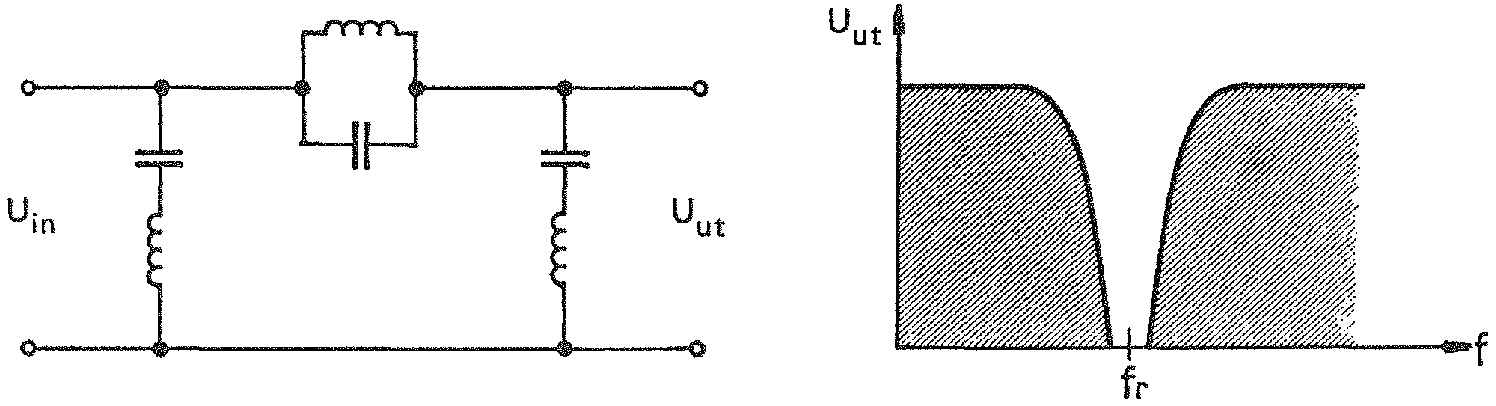
\includegraphics[width=\textwidth]{images/bild_2_3-26}
\caption{Bandspärrfilter}
\label{fig:BildII3-26}
\end{figure}

Bild \ref{fig:BildII3-26}

Om serie- och parallellkretsarna i ett bandpassfilter byter plats, så får man
i stället ett bandspärrfilter. Ett sådant spärrar signaler inom ett visst
frekvensområde, men släpper igenom signaler utom detta område.

\subsection{Spärrfilter}
\index{spärrfilter}
\index{filter!spärr (BR)}
\index{band reject filter (BR)}
\index{BR}
\index{spärrkrets}
\index{sugkrets}

\begin{figure}
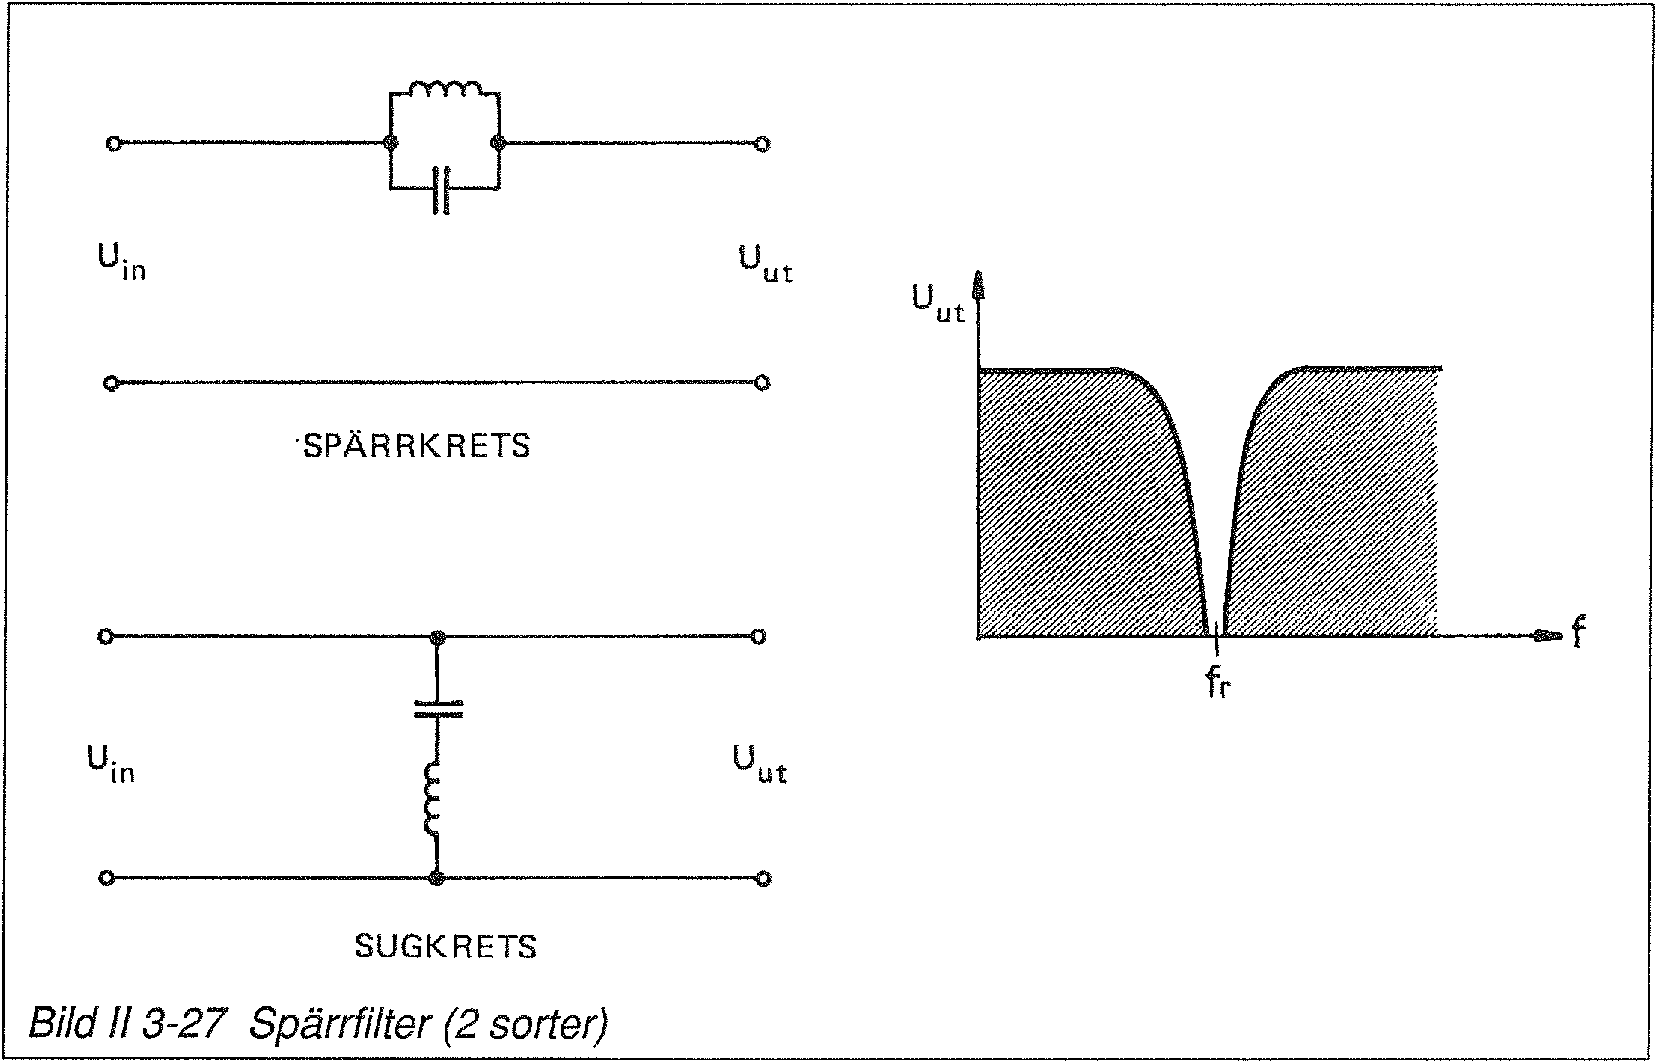
\includegraphics[width=\textwidth]{images/bild_2_3-27}
\caption{Spärrfilter (2 sorter)}
\label{fig:BildII3-27}
\end{figure}

Bild \ref{fig:BildII3-27}

\emph{Spärrkrets} \\
Spärrkretsen stäms av till en viss frekvens  och erbjuder där en mycket hög
impedans. Spärrkretsen kopplas i serie med signalvägen och spärrar en signal
med samma frekvens som resonansfrekvensen.

Bild \ref{fig:BildII3-27}

\emph{Sugkrets} \\
Sugkretsen stäms av till en viss frekvens och erbjuder där en mycket låg
impedans. Sugkretsen kopplas parallellt med signalvägen och kortsluter (suger
bort) en signal med samma frekvens som resonansfrekvensen.

\begin{wrapfigure}[14]{R}{0.5\textwidth}
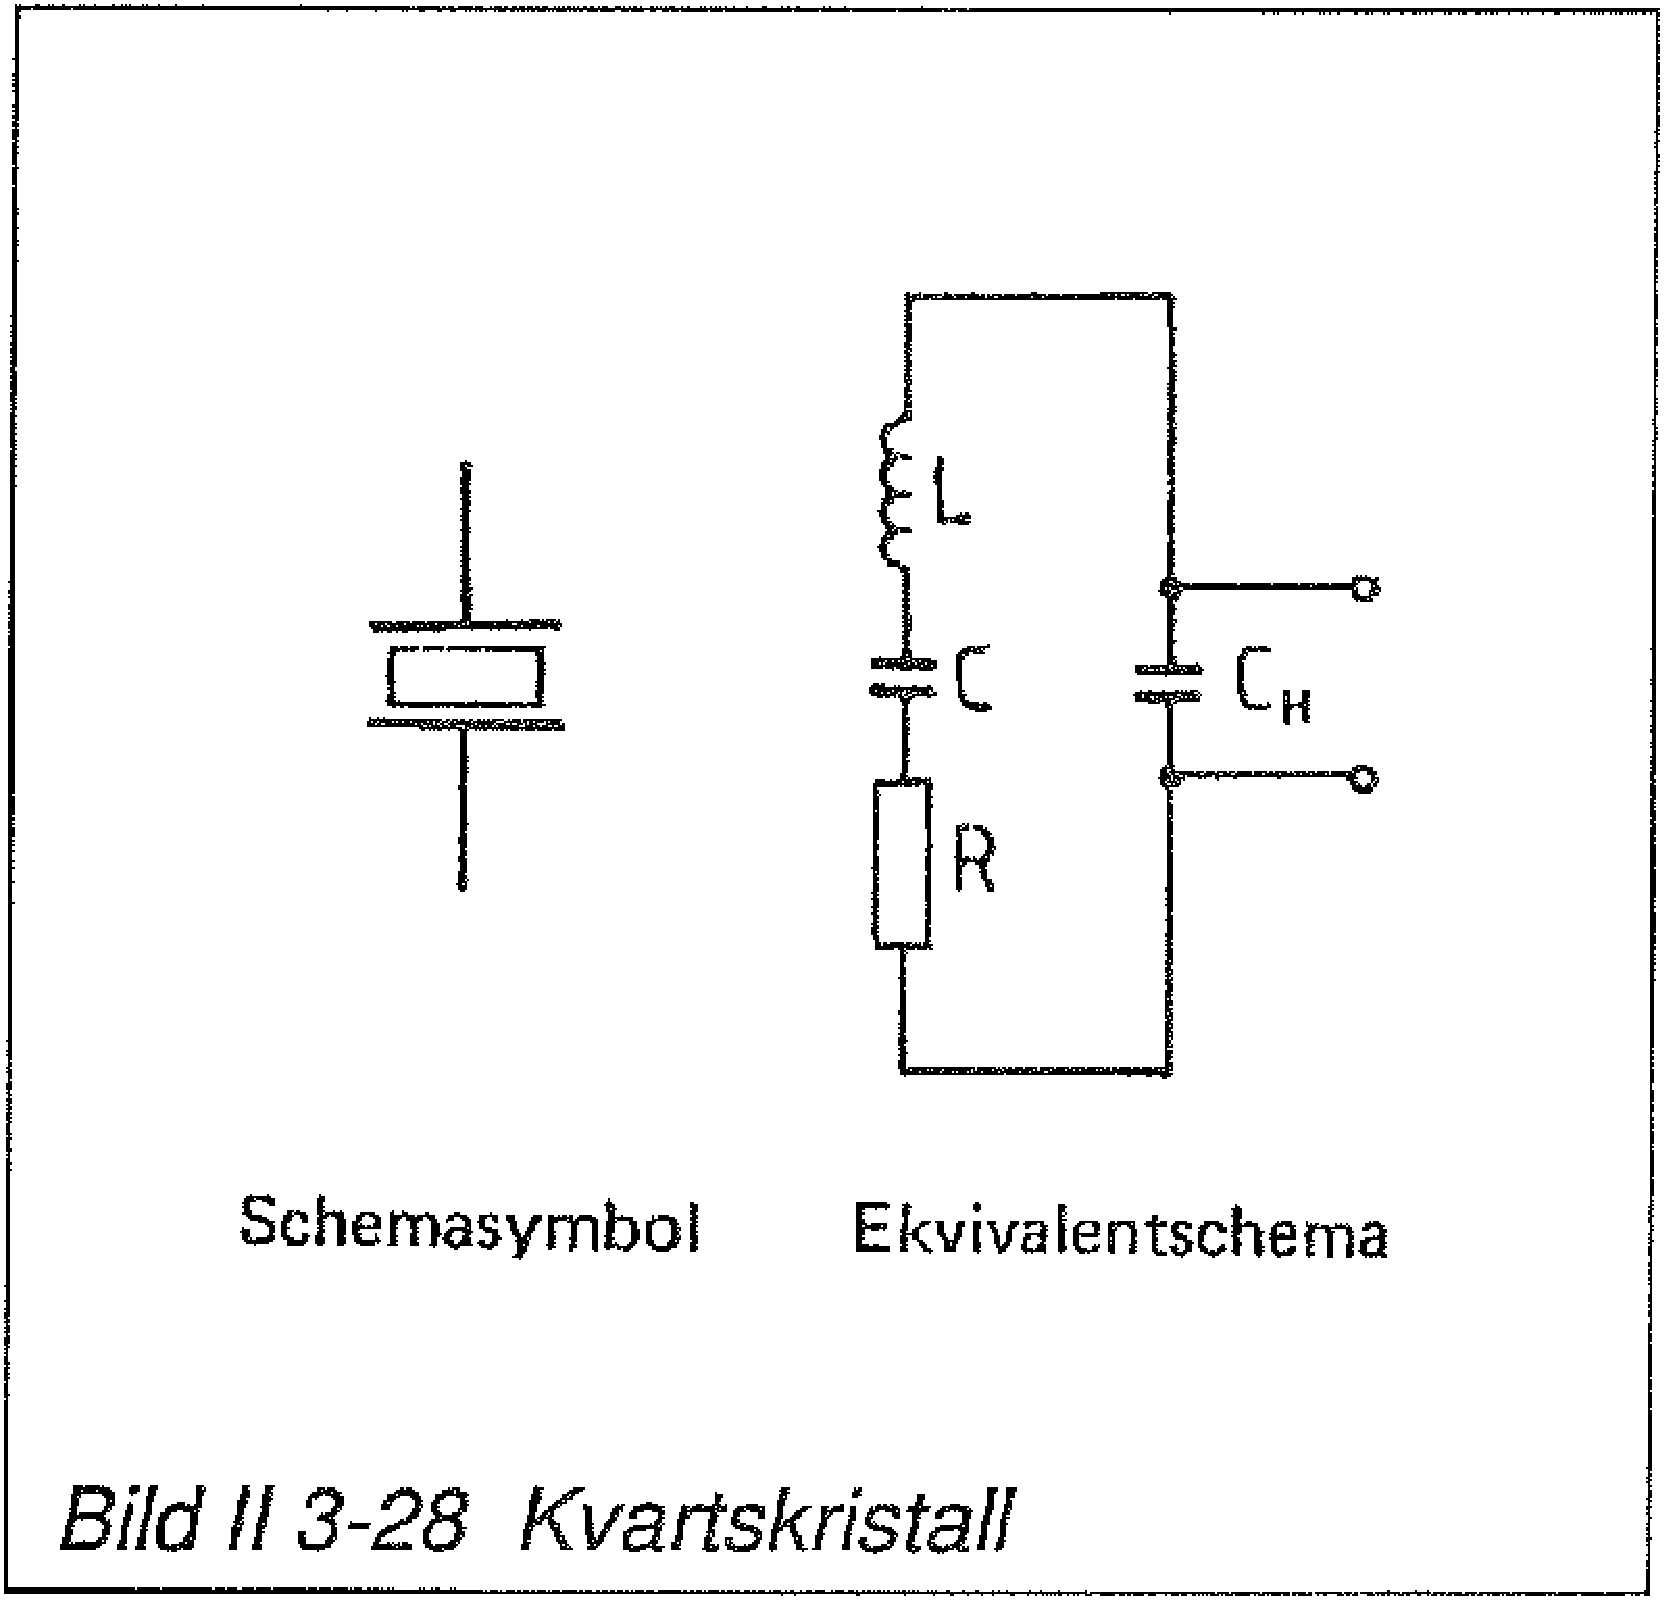
\includegraphics[width=0.5\textwidth]{images/bild_2_3-28}
\caption{Kvartskristall}
\label{fig:BildII3-28}
\end{wrapfigure}

\subsection{Kvartskristall}

\textbf{HAREC a.\ref{HAREC.a.3.2.11}\label{myHAREC.a.3.2.11}}
\index{kvartskristall}
\index{quartz crystal}
\index{crystal}
\index{Q-värde}
\index{resonator}

Bild \ref{fig:BildII3-28}

En \emph{kvartskristall} (eng \emph{quartz crystal} eller \emph{crystal}),
egentligen en slipad skiva av kvarts, kan fungera som en
elektromekanisk svängningskropp (resonator), vars egenskaper liknar dem i en
LC-krets.

Den låga inre resistansen gör att Q-värdet i en kvartskristall är bättre än
10000. Som jämförelse är Q-värdet i en LC-krets oftast sämre än 1000.

Många moderna kvartskristaller kan uppvisa olastat Q-värde på 100000.

\vspace{12pt} % Undgår brytning av nästa titelrad

\subsection{Bandfilter med kvartskristaller}
\index{kristallfilter}
\index{crystal filter}
\index{keramiska resonatorer}
\index{ceramic resonators}

\begin{wrapfigure}[17]{R}{0.5\textwidth}
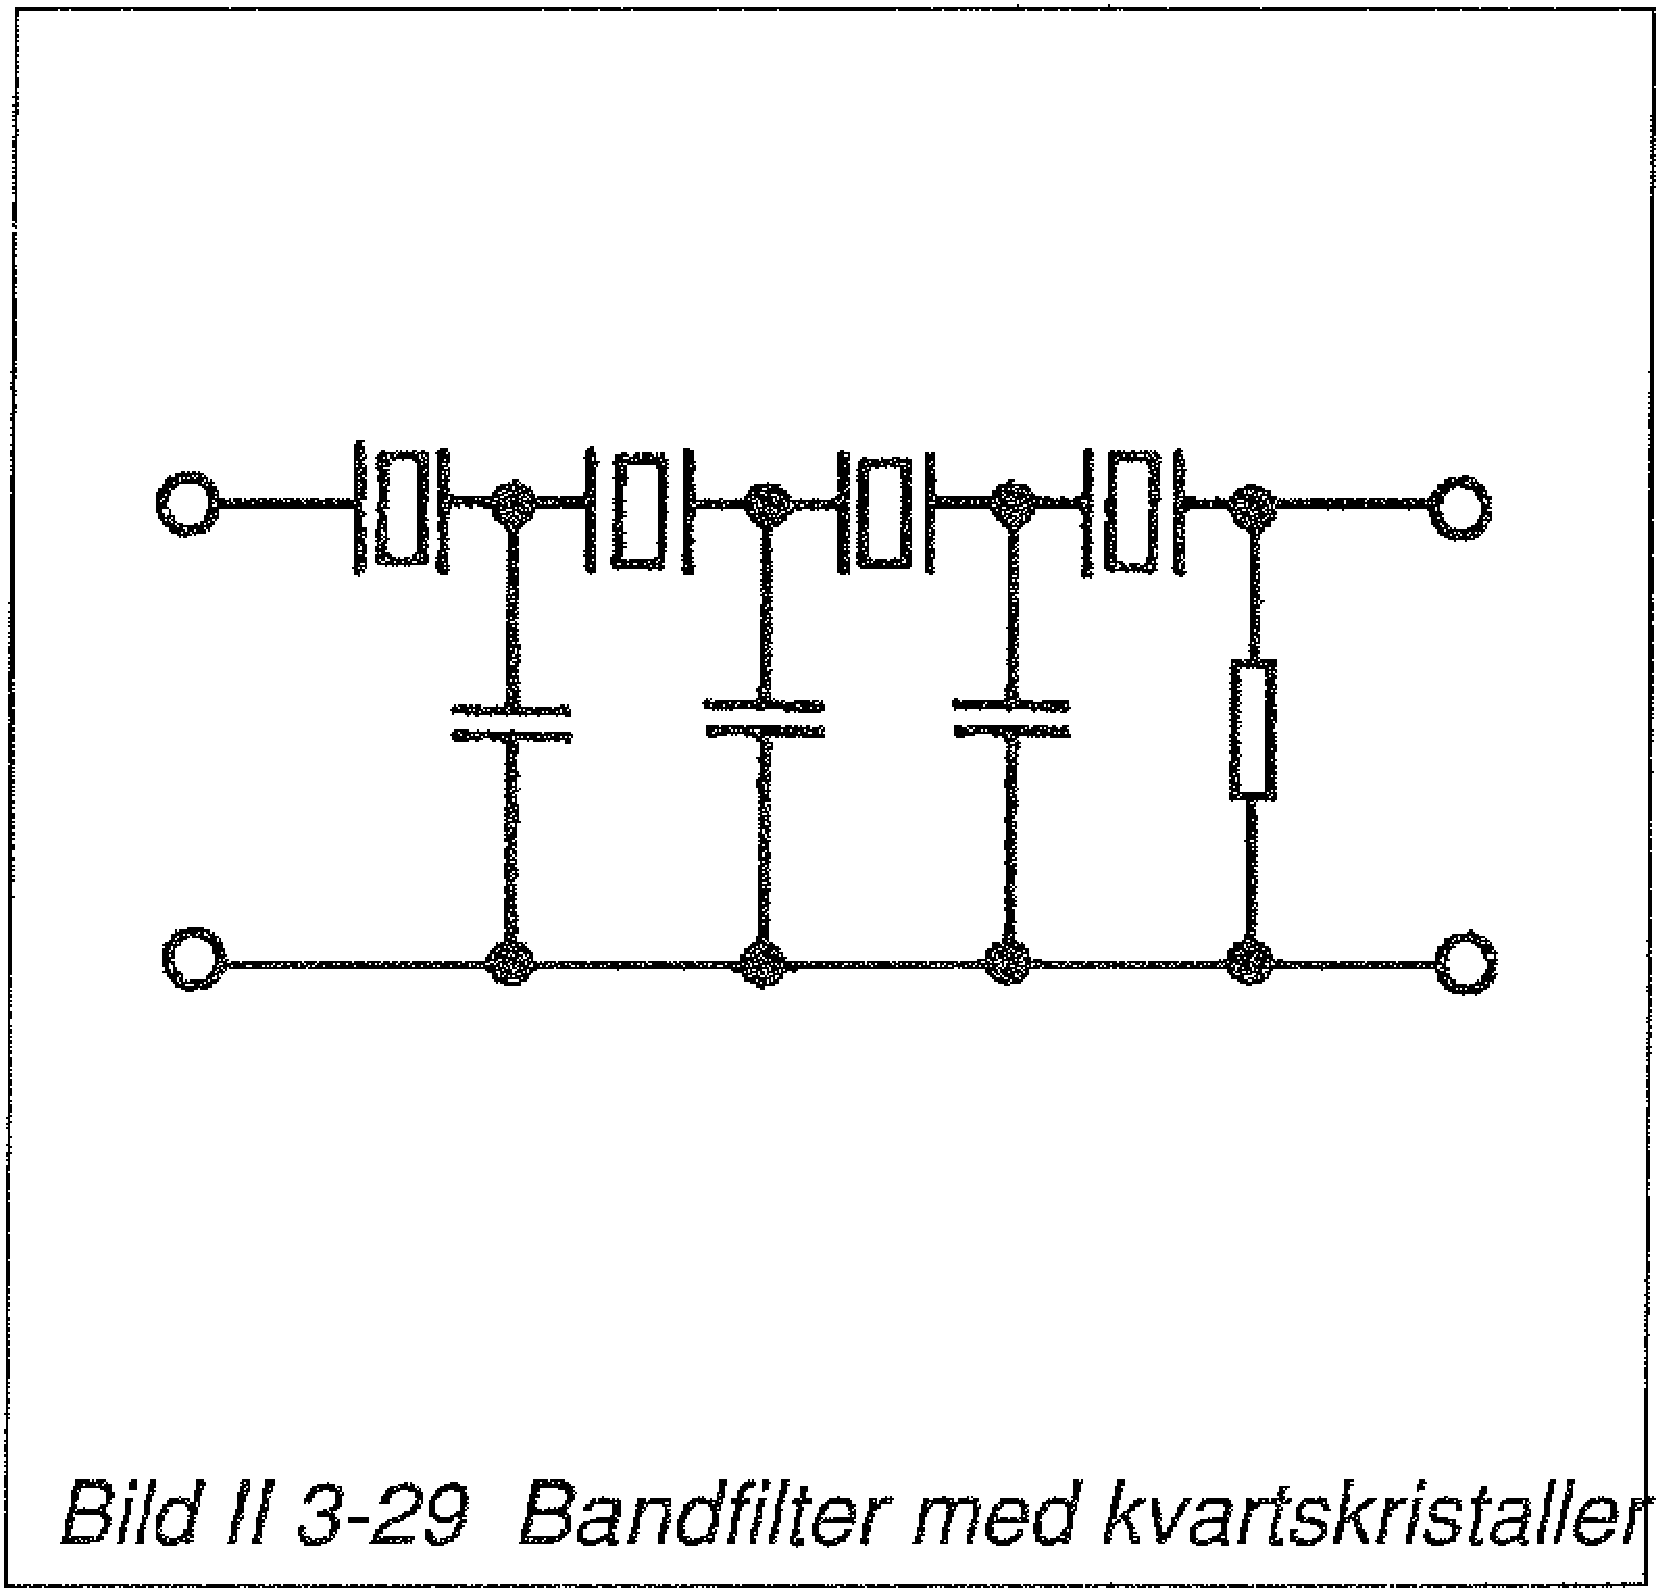
\includegraphics[width=0.5\textwidth]{images/bild_2_3-29}
\caption{Bandfilter med kvartskristaller}
\label{fig:BildII3-29}
\end{wrapfigure}

Bild \ref{fig:BildII3-29}

Kvartskristaller kan kombineras till filter, ofta refererade till som
\emph{kristallfilter} (eng \emph{crystal filter}), med önskad bandbredd. Även
utföranden med \emph{keramiska resonatorer} (eng \emph{ceramic resonators})
finns. Resonatorerna är avstämda till var sin bestämda frekvens och hela
komplexet bidrar på så sätt till att bilda passband eller andra egenskaper på
samma sätt som med sammankopplade LC-kretsar.

\subsection{Mekaniska filter}
\index{mekaniskt filter}
\index{mechanical filter}
\index{mekanisk resonator}
\index{resonator!mekanisk}

Bild \ref{fig:BildII3-30}

Med en elektromekanisk givare kan man få en kropp (resonator) att svänga på sin
resonansfrekvens. Med ännu en elektromagnetisk givare kan man känna av
svängningarna och återvandla dem till elektriska signaler. Hela anordningen
fungerar som en \emph{elektromekanisk resonator} (eng
\emph{mechanical resonator}), vars egenskaper liknar dem i en LC-krets.

\begin{figure}
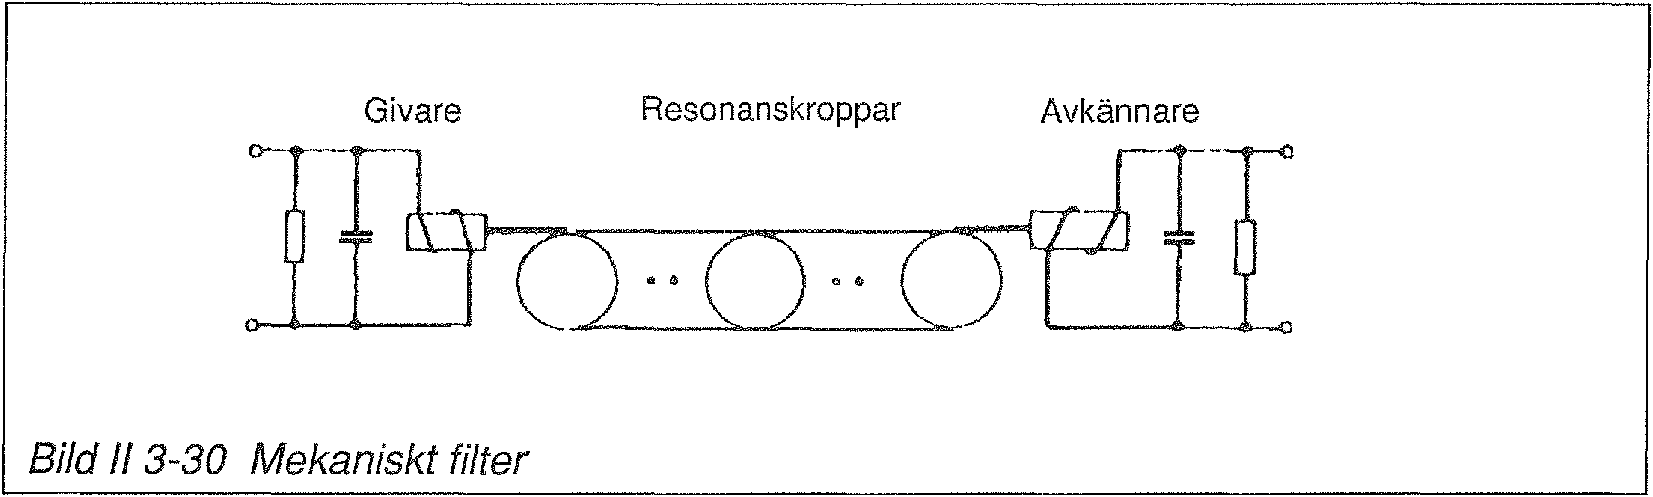
\includegraphics[width=\textwidth]{images/bild_2_3-30}
\caption{Mekaniskt filter}
\label{fig:BildII3-30}
\end{figure}

Resonatorerna kan kombineras till filterkomplex med önskad bandbredd där
resenatorerna är avstämda till var sin bestämda frekvens. Hela komplexet bidrar
på så sätt till att bilda ett passband på samma sätt som med sammankopplade
LC-kretsar. Beroende på tillämpningen finns olika frekvenslägen i intervallet
60--600~kHz.

\emph{Mekaniska filter} (eng \emph{mechanical filter}) användes mest förr som
mellanfrekvensfilter i högvärdiga radioutrustningar, men har numera till stor
del ersatts av bandfilter med kvartskristaller där arbetsområdet kan ligga
avsevärt högre i frekvens.

\subsection{Kavitetsfilter}
\index{kavitetsfilter}
\index{cavity filter}
\index{filter!kavitet}

\begin{wrapfigure}[15]{R}{0.5\textwidth}
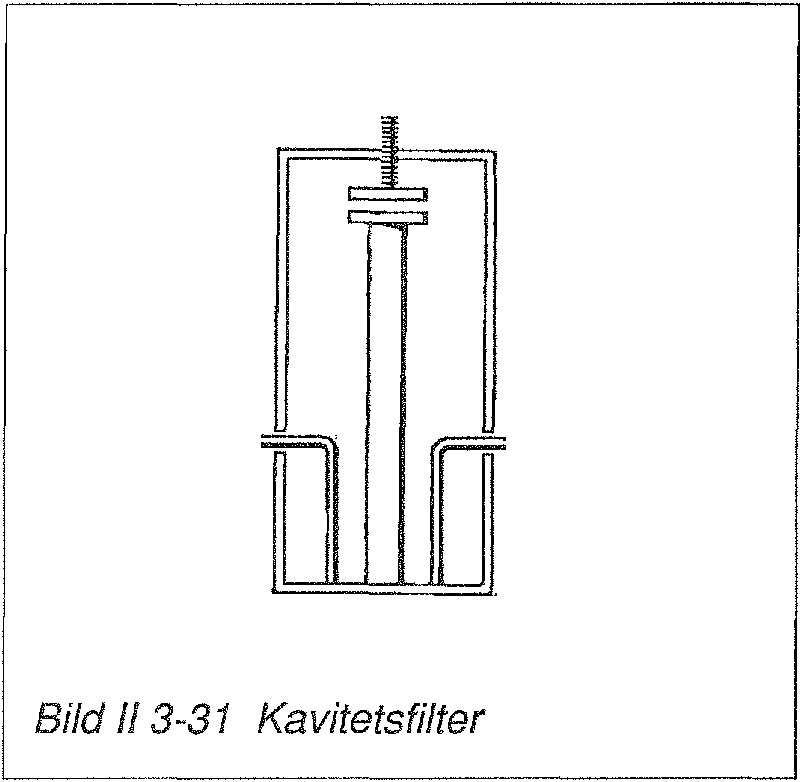
\includegraphics[width=0.5\textwidth]{images/bild_2_3-31}
\caption{Kavitetsfilter}
\label{fig:BildII3-31}
\end{wrapfigure}

Bild \ref{fig:BildII3-31}

Svängningskretsars dimensioner minskar med ökande frekvens. Vid mycket hög
frekvens kan induktorns varvtal i en LC-krets ha minskat till ett enda varv
samtidigt som kapacitansen inom detta enda varv kan räcka för önskad
resonansfrekvens.

En sådan svängningskrets kan bl.a. ha formen av en ledare mitt inne i en
elektriskt ledande kavitet. Ledarens längd tillsammans med kavitetens insida
bildar induktorn. Mellan ledaren och kavitetens insida råder en kapacitans,
som kan kompletteras/justeras med en extra kondensator.

Inkommande och utgående signaler ansluts till filtrets mittledare över
induktionsslingor, kondensatorer eller direkt galvaniskt. \emph{Kavitetsfilter} (eng
\emph{cavity filter}) kan kopplas ihop för att bilda bandfilter, frekvensdelare
m.m.

\subsection{Helixfilter}
\index{helixfilter}
%\index{helix filter}
\index{filter!helix}

När ett kompakt kavitetsfilter behövs, så kan man öka reaktansen i mittledaren
både induktivt och kapacitivt genom att utforma den som en spiral (helix).
Detta är dock på bekostnad av Q-värdet. Flera kavitetsfilter kan kopplas ihop
för att bilda bandfilter, spärrfilter m.m.

\subsection{Pi-filter}
\textbf{HAREC a.\ref{HAREC.a.3.2.10a}\label{myHAREC.a.3.2.10a}}
\index{Pi-filter}
\index{filter!Pi-filter}

\begin{wrapfigure}[16]{R}{0.5\textwidth}
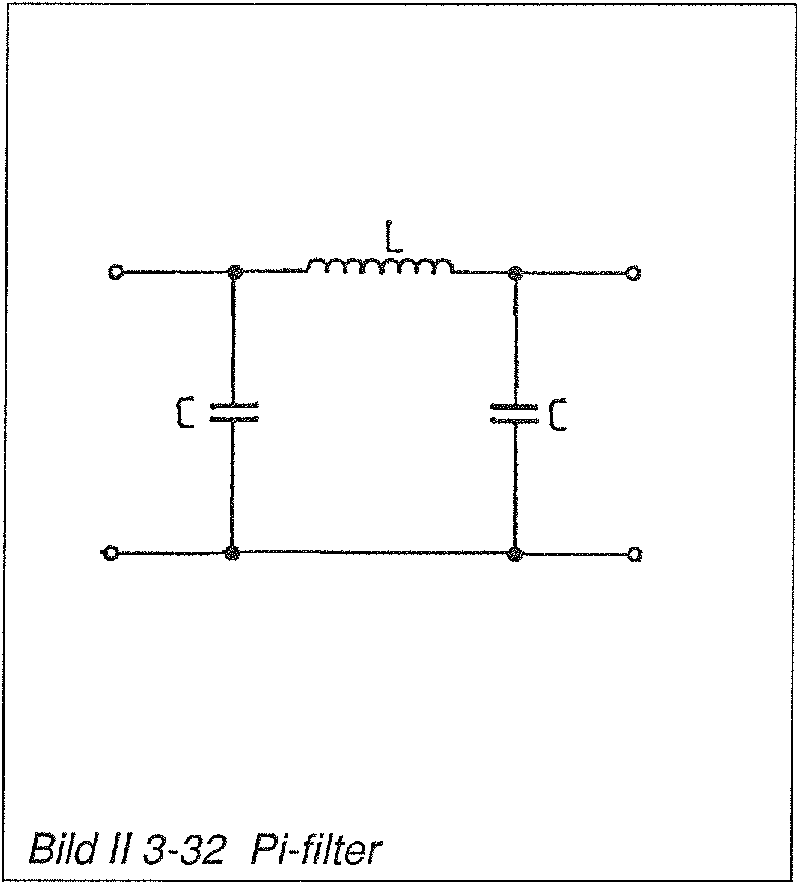
\includegraphics[width=0.5\textwidth]{images/bild_2_3-32}
\caption{Pi-filter}
\label{fig:BildII3-32}
\end{wrapfigure}

Bild \ref{fig:BildII3-32}

För att överföra HF-signaler med bästa verkningsgrad, så är det viktigt med god
impedansanpassning mellan de olika funktionerna. Om anslutningsimpedansen är
lika i båda funktionerna, så behövs inga extra åtgärder. Är impedanserna däremot
olika, så behövs korrigeringsnät (filter).

Ofta är nätet Pi-format och består av induktanser och kapacitanser. Ett
Pi-format nät kan sägas bestå av två L-formade nät ställda mot varandra, där
den seriella delen är gemensam (på bilden en induktor).

\subsection{T-filter}
\textbf{HAREC a.\ref{HAREC.a.3.2.10b}\label{myHAREC.a.3.2.10b}}
\index{T-filter}
\index{filter!T-filter}

\begin{wrapfigure}[16]{R}{0.5\textwidth}
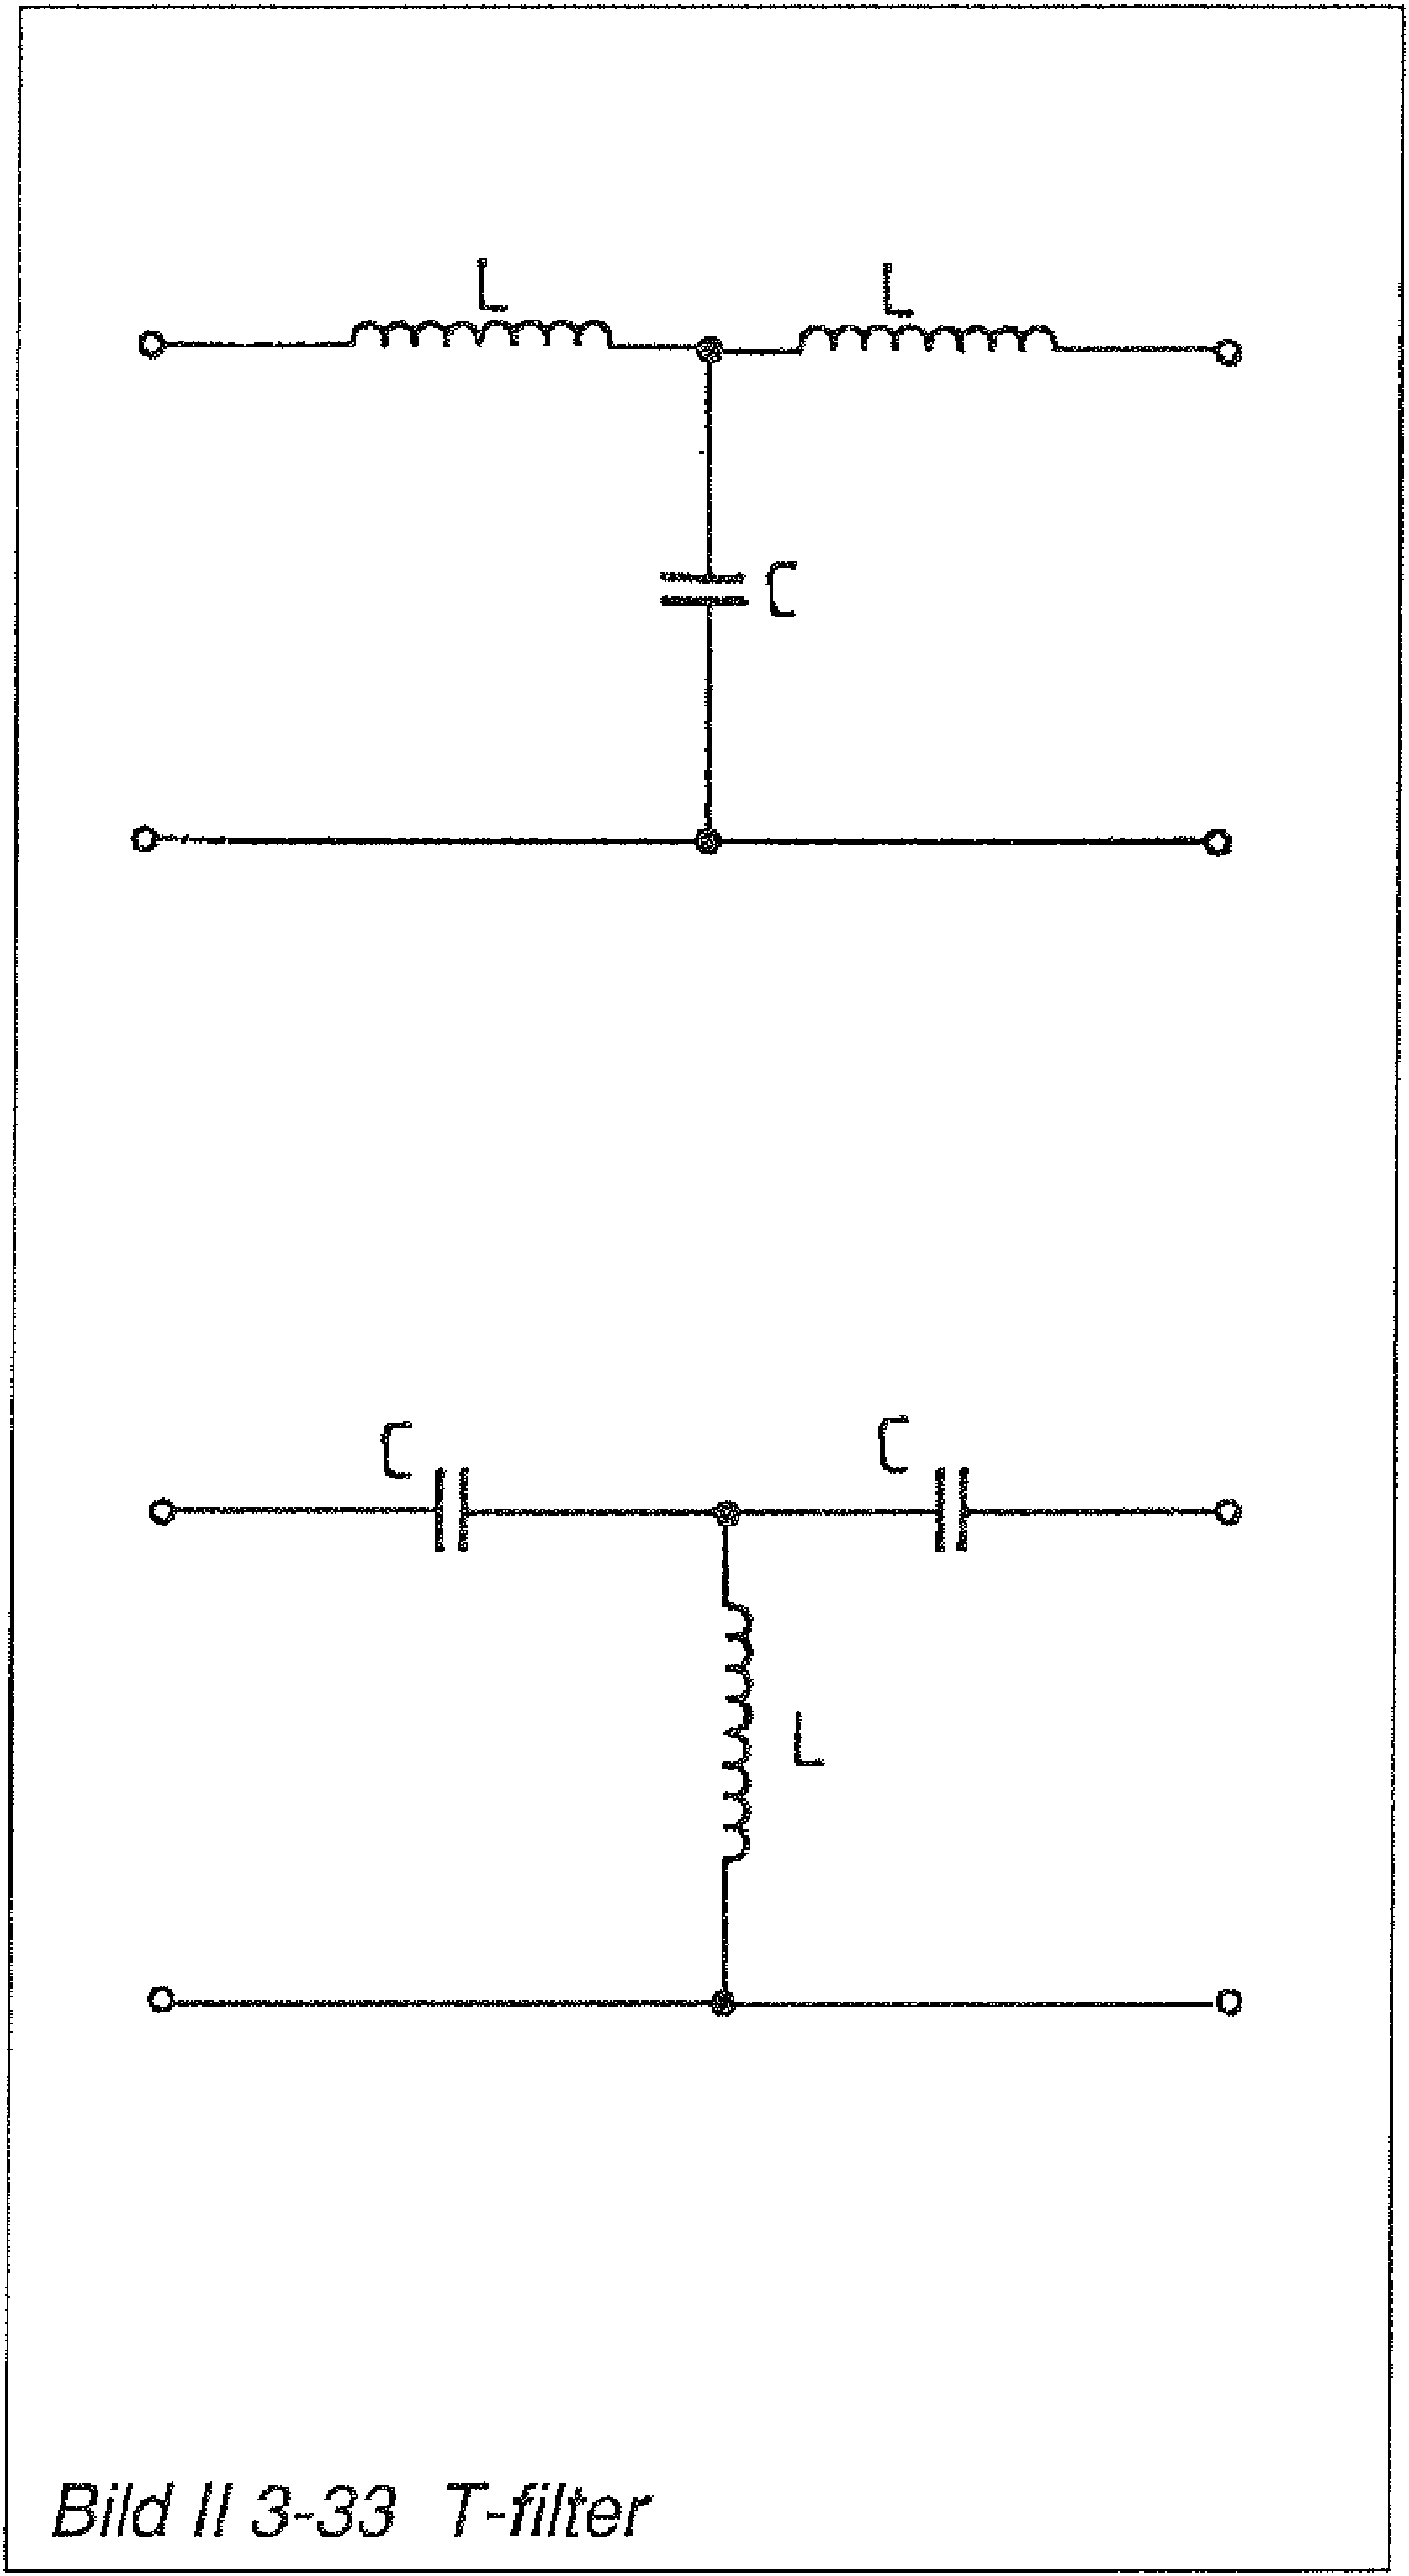
\includegraphics[width=0.5\textwidth]{images/bild_2_3-33}
\caption{T-filter}
\label{fig:BildII3-33}
\end{wrapfigure}

Bild \ref{fig:BildII3-33}

Ett nät kan också vara T-format och bestå av induktanser och kapacitanser. Ett
sådant nät kan sägas bestå av två L-formade nät ställda ''rygg mot rygg''. Då är
den parallella delen gemensam. På bilden visas två alternativ.

När den parallella delen är kapacitiv, blir huvudkaraktären ett lågpassfilter,
men att impedansanpassning också är möjlig med en induktiv impedansdelning.

När den parallell delen är induktiv blir huvudkaraktären ett högpassfilter, men
att impedansanpassning också är möjlig med en kapacitiv impedansdelning.

Ett Pi- eller T-filter kan fungera som
\begin{itemize}
\item svängningskrets,
\item impedanstransformator (anpassning),
\item balansera ut en reaktans o.s.v.
\end{itemize}
